\documentclass[12pt,landscape]{article}
\usepackage{multicol}
\usepackage{calc}
\usepackage{ifthen}
\usepackage[landscape]{geometry}
\usepackage{hyperref}
\usepackage{graphicx}
\graphicspath{ {./img/} }
\usepackage{wrapfig}
\usepackage{amsmath}
% This sets page margins to .5 inch if using letter paper, and to 1cm
% if using A4 paper. (This probably isn't strictly necessary.)
% If using another size paper, use default 1cm margins.
\ifthenelse{\lengthtest { \paperwidth = 11in}}
	{ \geometry{top=.5in,left=.5in,right=.5in,bottom=.5in} }
	{\ifthenelse{ \lengthtest{ \paperwidth = 297mm}}
		{\geometry{top=1cm,left=1cm,right=1cm,bottom=1cm} }
		{\geometry{top=1cm,left=1cm,right=1cm,bottom=1cm} }
	}

% Turn off header and footer


% \pagestyle{empty}
 

% Redefine section commands to use less space
\makeatletter
\renewcommand{\section}{\@startsection{section}{1}{0mm}%
                                {-1ex plus -.5ex minus -.2ex}%
                                {0.5ex plus .2ex}%x
                                {\normalfont\large\bfseries}}
\renewcommand{\subsection}{\@startsection{subsection}{2}{0mm}%
                                {-1explus -.5ex minus -.2ex}%
                                {0.5ex plus .2ex}%
                                {\normalfont\normalsize\bfseries}}
\renewcommand{\subsubsection}{\@startsection{subsubsection}{3}{0mm}%
                                {-1ex plus -.5ex minus -.2ex}%
                                {1ex plus .2ex}%
                                {\normalfont\small\bfseries}}
\makeatother

% Define BibTeX command
\def\BibTeX{{\rm B\kern-.05em{\sc i\kern-.025em b}\kern-.08em
    T\kern-.1667em\lower.7ex\hbox{E}\kern-.125emX}}

% Don't print section numbers
\setcounter{secnumdepth}{0}


\setlength{\parindent}{0pt}
\setlength{\parskip}{0pt plus 0.5ex}


% -----------------------------------------------------------------------

\begin{document}

\raggedright
\footnotesize
\begin{multicols}{3}


% multicol parameters
% These lengths are set only within the two main columns
%\setlength{\columnseprule}{0.25pt}
\setlength{\columnseprule}{0.25pt}
\setlength{\premulticols}{0.25pt}
\setlength{\postmulticols}{0.25pt}
\setlength{\multicolsep}{0.25pt}
\setlength{\columnsep}{0.25pt}

\begin{center}
     \Large{{Lineare Algebra Semester 2}} \\
\end{center}


\section{Vektorgeometrie}
\subsection{Betrag}
$\mid \vec{a} \mid  $ = $
\begin{pmatrix}
x\\
y\\
z
\end{pmatrix}$ = $ \sqrt[]{x^2+y^2+z^2}$
\\
\subsection{Skalarprodukt}
$  \vec{a} \cdot \vec{b} =  \begin{pmatrix}
a_x\\
a_y\\
a_z
\end{pmatrix} \cdot \begin{pmatrix}
b_x\\
b_y\\
b_z
\end{pmatrix} = a_xb_x+a_yb_y+a_zb_z$

$ \vec{a} \cdot \vec{b} $ = $ \mid \vec{a} \mid \cdot \mid \vec{b} \mid \cdot \cos(\varphi)$
\section{Document classes}
\begin{wrapfigure}{r}{0.45\linewidth}
    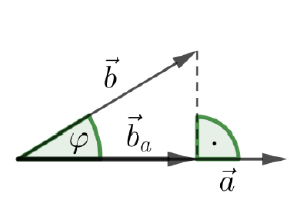
\includegraphics[scale=0.25]{ortho.png} 

\end{wrapfigure}
asdasdasdasdasd asdasdasda sdasdasdasdasda sdasdasdasd asdasdasd

Used at the very beginning of a document:
\verb!\documentclass{!\textit{class}\verb!}!.  Use
\verb!\begin{document}! to start contents and \verb!\end{document}! to
end the document.





\end{multicols}
\end{document}
